%% 
%% Copyright 2007-2020 Elsevier Ltd
%% 
%% This file is part of the 'Elsarticle Bundle'.
%% ---------------------------------------------
%% 
%% It may be distributed under the conditions of the LaTeX Project Public
%% License, either version 1.2 of this license or (at your option) any
%% later version.  The latest version of this license is in
%%    http://www.latex-project.org/lppl.txt
%% and version 1.2 or later is part of all distributions of LaTeX
%% version 1999/12/01 or later.
%% 
%% The list of all files belonging to the 'Elsarticle Bundle' is
%% given in the file `manifest.txt'.
%% 
%% Template article for Elsevier's document class `elsarticle'
%% with harvard style bibliographic references

\documentclass[preprint,12pt]{elsarticle}

%% Use the option review to obtain double line spacing
%% \documentclass[preprint,review,12pt]{elsarticle}

%% Use the options 1p,twocolumn; 3p; 3p,twocolumn; 5p; or 5p,twocolumn
%% for a journal layout:
%% \documentclass[final,1p,times]{elsarticle}
%% \documentclass[final,1p,times,twocolumn]{elsarticle}
%% \documentclass[final,3p,times]{elsarticle}
%% \documentclass[final,3p,times,twocolumn]{elsarticle}
%% \documentclass[final,5p,times]{elsarticle}
%% \documentclass[final,5p,times,twocolumn]{elsarticle}

%% For including figures, graphicx.sty has been loaded in
%% elsarticle.cls. If you prefer to use the old commands
%% please give \usepackage{epsfig}

%% The amssymb package provides various useful mathematical symbols
\usepackage{amssymb}
%% The amsthm package provides extended theorem environments
\usepackage{amsthm}

\newtheorem{theorem}{Theorem}[section]
\newtheorem{example}{Example}[section]
\newtheorem{definition}{Definition}[section]
\newtheorem{proposition}{Proposition}[section]

%% The lineno packages adds line numbers. Start line numbering with
%% \begin{linenumbers}, end it with \end{linenumbers}. Or switch it on
%% for the whole article with \linenumbers.
\usepackage{lineno}

\usepackage{hyperref}

%%%%%%%%%%%%%%%%%%%%%%%%%%%%%%%%%%%%%%%%%%%%%%%%%%%%%%%%%%%%
%% Drawing
%%%%%%%%%%%%%%%%%%%%%%%%%%%%%%%%%%%%%%%%%%%%%%%%%%%%%%%%%%%%
\usepackage{tikz}
\usepackage{amsfonts}

% drawing automa
\usetikzlibrary{positioning,automata}

% for captions in figures
\usepackage[labelformat=simple]{subcaption}
\renewcommand\thesubfigure{(\alph{subfigure})}

\usepackage{booktabs}

% table row numbers
\newcounter{rownumber}
\newcommand\rownb{\stepcounter{rownumber}\arabic{rownumber}}

\newcommand{\vangiang}[1]{\textcolor{magenta}{#1}}
\newcommand{\belaid}[1]{\textcolor{blue}{#1}}
\newcommand{\sylvain}[1]{\textcolor{teal}{#1}}

\journal{Theoretical Computer Science}

\begin{document}

\begin{frontmatter}

%% Title, authors and addresses

%% use the tnoteref command within \title for footnotes;
%% use the tnotetext command for theassociated footnote;
%% use the fnref command within \author or \address for footnotes;
%% use the fntext command for theassociated footnote;
%% use the corref command within \author for corresponding author footnotes;
%% use the cortext command for theassociated footnote;
%% use the ead command for the email address,
%% and the form \ead[url] for the home page:
%% \title{Title\tnoteref{label1}}
%% \tnotetext[label1]{}
%% \author{Name\corref{cor1}\fnref{label2}}
%% \ead{email address}
%% \ead[url]{home page}
%% \fntext[label2]{}
%% \cortext[cor1]{}
%% \affiliation{organization={},
%%             addressline={},
%%             city={},
%%             postcode={},
%%             state={},
%%             country={}}
%% \fntext[label3]{}

\title{Minimal trap spaces of Boolean networks are maximal siphons of their Petri net encoding}

%% use optional labels to link authors explicitly to addresses:
%% \author[label1,label2]{}
%% \affiliation[label1]{organization={},
%%             addressline={},
%%             city={},
%%             postcode={},
%%             state={},
%%             country={}}
%%
%% \affiliation[label2]{organization={},
%%             addressline={},
%%             city={},
%%             postcode={},
%%             state={},
%%             country={}}

\author{Van-Giang Trinh\fnref{1}}
\ead{trinh.van-giang@lis-lab.fr}

\author{Belaid Benhamou\fnref{1}}
\ead{belaid.benhamou@lis-lab.fr}

\affiliation[1]{organization={LIS, Aix-Marseille University},%Department and Organization
            %addressline={}, 
            city={Marseille},
            %postcode={}, 
            %state={},
            country={France}}

\author{Sylvain Soliman\corref{cor1}\fnref{2}}
\ead{Sylvain.Soliman@inria.fr}

\affiliation[2]{organization={Lifeware team, Inria Saclay center},%Department and Organization
            %addressline={}, 
            city={Palaiseau},
            %postcode={}, 
            %state={},
            country={France}}

\cortext[cor1]{Corresponding author.}

\begin{abstract}
%% Text of abstract

Boolean modeling of gene regulation but also of post-trans\-criptomic systems has proven over the years that it can bring powerful analyses and corresponding insight to the many cases where precise biological data is not sufficiently available to build a detailed quantitative model.
This is even more true for very large models where such data is frequently missing and led to a constant increase in size of logical models \emph{à la} Thomas.
Besides simulation, the analysis of such models is mostly based on attractor computation, since those correspond roughly to observable biological \emph{phenotypes}. The recent use of trap spaces made a real breakthrough in that field allowing to consider medium-sized models that used to be out of reach.
However, with the continuing increase in model-size, the state-of-the-art computation of minimal trap spaces based on \emph{prime-implicants} shows its limits as there can be a huge number of implicants.

In this article we present an alternative method to compute minimal trap spaces, and hence complex attractors, of a Boolean network. It replaces the need for prime-implicants by a completely different technique, namely the enumeration of maximal siphons in the Petri net encoding of the original model.
After some technical preliminaries, we expose the concrete need for such a method and detail its implementation using Answer Set Programming.
We then demonstrate its efficiency and compare it to implicant-based methods on some large Boolean networks from the literature.
  
\end{abstract}

%%Graphical abstract
% \begin{graphicalabstract}
% %\includegraphics{grabs}
% \end{graphicalabstract}

%%Research highlights
% \begin{highlights}
% \item Research highlight 1
% \item Research highlight 2
% \end{highlights}

\begin{keyword}
%% keywords here, in the form: keyword \sep keyword

%% PACS codes here, in the form: \PACS code \sep code

%% MSC codes here, in the form: \MSC code \sep code
%% or \MSC[2008] code \sep code (2000 is the default)

Logical model \sep Boolean network \sep Trap space \sep Attractor computation \sep Petri net \sep Siphon \sep Answer set programming \sep Systems biology
\end{keyword}

\end{frontmatter}

\linenumbers

%% main text
\section{Introduction}

From the observation that the transcriptional regulation behaved in a sigmoid step-like way, came the original idea to represent models of gene regulation as discrete event systems.
Those Gene Regulation Networks (GRN) use thresholds or equivalently logical functions to represent the different regulations~\cite{glass1973logical,thomas1973boolean,thomas1990biological,thomas1991regulatory}.

Boolean modelling has proven over the years that it can bring powerful analyses and corresponding insight to the many cases where precise biological data is not sufficiently available to build a detailed quantitative model~\cite{wang2012boolean}, even for modelling post-transcriptional mechanisms.
This is even more true for very large models where such data is frequently missing and led to a constant increase in size of logical models \emph{à la} Thomas~\cite{aghamiri2020automated}.
Besides simulation, the analysis of such models is mostly based on attractor computation, since those correspond roughly to observable biological \emph{phenotypes}.
The recent use of trap spaces~\cite{klarner2015computing} made a real breakthrough in that field allowing to consider medium-sized models that used to be out of reach.
However, with the continuing increase in model-size, the state-of-the-art computation of minimal trap spaces based on \emph{prime-implicants} shows its limits as there can be a huge number of implicants.

It is worth noting that the recent method presented in~\cite{DBLP:conf/ictai/ChevalierFPZ19} for computing minimal trap spaces avoids the prime-implicants computation by relying on the \emph{most-permissive} semantics of Boolean networks.
This method has been implemented in the tool mpbn\footnote{\url{https://github.com/bnediction/mpbn}} demonstrated in~\cite{Paulev2020} for handling medium-sized models from the literature and very large synthetic models (up to 100,000 nodes).
However, this method is only applicable for \emph{locally-monotonic} Boolean networks, whereas the prime-implicants based method~\cite{klarner2015computing} is applicable for \emph{general} Boolean networks (i.e., including both locally-monotonic and non-locally-monotonic ones).
The study~\cite{DBLP:journals/tcs/NoualRS13} highlights the need for non-locally-monotonic Boolean networks in both biological and theoretical aspects.
Hence, it is still necessary to develop efficient methods for computing minimal trap spaces of large-scale general Boolean networks.

Petri nets were introduced in the 60s as simple formalism for describing and analyzing information-processing systems that are characterized as being concurrent, asynchronous, non-deterministic and possibly distributed~\cite{peterson1981petri,Murata1989}.
The use of Petri nets for representing biochemical reaction systems, by mapping molecular species to places and reactions to transitions, hinted at already in~\cite{peterson1981petri,Murata1989} was used more thoroughly quite late in~\cite{reddy1993petri}, together with some Petri net concepts and tools for the analysis of metabolic networks.
Siphons are such a concept, but they have not been used a lot for the study of biochemical systems~\cite{zevedei2003topological,blatke2015biomodel} even if the practical cost of computing their minimal/maximal elements appear much more manageable than the theoretical complexity would indicate~\cite{oanea2010new,nabli2016enumerating}.

In this article we present an alternative method to compute minimal trap spaces, and hence complex attractors, of a general Boolean network. It replaces the need for prime-implicants by a completely different technique, namely the enumeration of maximal siphons in the Petri net encoding of the original model (Section~\ref{sec:Main_finding}).
After some technical preliminaries (Section~\ref{sec:Preliminaries}), we expose the concrete need for such a method and detail its implementation using Answer Set Programming (Section~\ref{sec:Computation}).
We then demonstrate its efficiency and compare it to implicant-based methods on several large Boolean networks from the literature (Section~\ref{sec:eval}).

All models used for evaluation and the implementation of the presented method are available at \url{https://github.com/soli/trap-spaces-as-siphons} and executable as a CoLoMoTo docker image.

% Mention the extensions for the journal version
Herein we extend our previous work in~\cite{DBLP:conf/cmsb/TrinhBHS22} as follows.
First, we showcase one theoretical application of the connection between trap spaces in Boolean networks and conflict-free siphons in Petri nets.
Second, beyond the proposed ASP method, we propose several other possible methods using MaxSAT, CLP, and ILP.
Third, we conduct a more comprehensive benchmark on both real-world and randomly generated models to evaluate all the proposed methods.
Forth, regarding the implementation, we have developed a converter that directly reads a .bnet file and builds the Petri net encoding, instead of using the PNML conversion of BioLQM.
Finally, we explore several complexity analysis on maximal (conflict-free) siphon problems.

\section{Preliminaries}
\label{sec:Preliminaries}

We shall briefly recall here some preliminaries on Boolean networks related to trap spaces and Petri nets.
In the case of multi-level logical models, an encoding into a Boolean network is always possible~\cite{Didier2011}.

\subsection{Boolean networks}

\begin{definition}

  A Boolean Network (BN) is a pair \(\mathcal{N} = (V, F)\) where:
  \begin{itemize}
    \item \(V = \{v_1, \dots, v_n\}\) is the set of nodes.
    We use \(v_i\) to denote both the node \(v_i\) and its associated Boolean variable.
    
    \item \(F = \{f_1, \dots, f_n\}\) is the set of update functions.
    Each function \(f_i\) is associated with node \(v_i\) and satisfies \(f_i \colon \mathbb{B}^{\vert IN(v_i)\vert} \mapsto \mathbb{B}\) where \(\mathbb{B} = \{0, 1\}\) and \(IN(v_i)\) denotes the set of input nodes of \(v_i\).
  \end{itemize}

\label{def:BN}
\end{definition}

A Boolean function is \emph{locally-monotonic} if it can be represented by a formula in disjunctive normal form in which all occurrences of any given literal are either negated or non-negated~\cite{Paulev2020}.
A Boolean network is said to be locally-monotonic if all its Boolean functions are locally-monotonic. 
Otherwise, this model is said to be non-locally-monotonic.

A state \(v \in \mathbb{B}^{n}\) is as a mapping \(v \colon V \mapsto \mathbb{B}\) that assigns either 0 (inactive) or 1 (active) to each node.
We denote the set of all possible states of a Boolean network \(\mathcal{N}\) by \(\mathcal{S}_{\mathcal{N}} = \mathbb{B}^n\).
At each time step \(t\), node \(v_i\) can update its state by
\[v_i(t + 1) = f_i(v(t))\]
where \(v(t)\) is the state of \(\mathcal{N}\) at time \(t\) and \(v_i(t + 1)\) is the state of node \(v_i\) at time \(t + 1\).
Note that for simplicity, we write \(f_i(v(t))\) even \(IN(v_i) \subset V\).
An update scheme of a Boolean network specifies the way that the nodes update their states through time evolution~\cite{thomas1991regulatory}. 
Following the update scheme, the Boolean network transits from a state to another state (possibly identical).
This transition is called the \emph{state transition} and denoted by \(\rightarrow \subseteq \mathcal{S}_{\mathcal{N}} \times \mathcal{S}_{\mathcal{N}}\).
Then the dynamics of \(\mathcal{N}\) is captured by the directed graph \((\mathcal{S}_{\mathcal{N}}, \rightarrow)\) called the State Transition Graph (STG).
There are two main types of update schemes~\cite{thomas1991regulatory}: synchronous, where all the nodes are update simultaneously, and fully asynchronous, where only one node is nondeterministically selected to be updated.

\subsection{Traps spaces}

We recall here some definitions from~\cite{klarner2015computing} for the introduction of \emph{trap spaces}.
Minimal trap spaces prove to be a very good approximation of the attractors of a Boolean network under asynchronous update schemes and have become the \emph{de facto} standard way to analyze models of a few tens of \emph{genes}~\cite{klarner2017pyboolnet,cifuentes2020control}.

An non-empty set \(T \subseteq \mathcal{S}_{\mathcal{N}}\) is a trap set with respect to \(\rightarrow\) if for every \(x \in T\) and \(y \in S\) with \(x \rightarrow y\) it holds that \(y \in T\)~\cite{klarner2015computing}.
An attractor of \(\mathcal{N}\) with respect to \(\rightarrow\) can be defined as an inclusion-wise minimal trap set of \((\mathcal{S}_{\mathcal{N}}, \rightarrow)\).
An attractor can be also seen as a terminal strongly connected component of \((\mathcal{S}_{\mathcal{N}}, \rightarrow)\)~\cite{chatain2014characterization}.
An attractor of size 1 is called a fixed point, otherwise a cyclic attractor~\cite{klarner2015computing}.

A subspace \(m\) of a Boolean network \(\mathcal{N} = (V, F)\) is a mapping \(m \colon V \mapsto \mathbb{B} \cup \{\star\}\).
\(m(v_i) \in \mathbb{B}\) means that the value of \(v_i\) is fixed in \(m\) and \(v_i\) is called a fixed variable.
\(m(v_i) \in \star\) means that the value of \(v_i\) is free in \(m\) and \(v_i\) is called a free variable.
We denote \(D_m\) the set of all fixed variables of \(m\).
A subspace \(m\) is equivalent to a set of states:
\[
\mathcal{S}_{\mathcal{N}}[m] := \{s \in \mathcal{S}_{\mathcal{N}} \mid \forall v \in D_m \colon s(v) = m(v)\}.
\] For example, \(m = \star\star1\) (for simplicity, we write subspaces likes states) means that \(D_m = \{v_3\}, m(v_3) = 1\), and it is equivalent to the set of states \(\{001, 011, 101, 111\}\).
We denote \(\mathcal{S}_{\mathcal{N}}^{\star} = (\mathbb{B} \cup \{\star\})^n\) the set of all possible subspaces of \(\mathcal{N}\).
Note that \(\left\vert\mathcal{S}_{\mathcal{M}}^{\star}\right\vert = 3^n\) and \(S_{\mathcal{N}} \subset \mathcal{S}_{\mathcal{N}}^{\star}\)~\cite{klarner2015computing}.

A \emph{trap space} is defined as a subspace that is also a trap set.
It is noted that trap spaces of a Boolean network are independent of the update scheme of this model~\cite{klarner2015computing}.
Then, we define a partial order \(<\) on \(\mathcal{S}_{\mathcal{N}}^{\star}\) as: \(m < m'\) if and only if \(\mathcal{S}_{\mathcal{N}}[m] \subseteq \mathcal{S}_{\mathcal{N}}[m']\) and \(\mathcal{S}_{\mathcal{N}}[m] \neq \mathcal{S}_{\mathcal{N}}[m']\).
Consequently, a trap space \(m\) is minimal if and only if there is no trap space \(m' \in \mathcal{S}_{\mathcal{N}}^{\star}\) such that \(m' < m\).

For example, let us consider the Boolean network shown in Example~\ref{example:BN}.
Figure~\ref{fig:stg} shows the dynamics of this model under the fully asynchronous update (i.e., only one node is nondeterministically selected in order to be updated at each time step).
The model has all two trap spaces, \(m_1 = 11\) and \(m_2 = \star\star\).
Since \(m_1 < m_2\), \(m_1\) is a minimal trap space of the Boolean network.

\begin{example}
We give a Boolean network \(\mathcal{M} = (V, F)\), where \(V = (x_1, x_2)\) and \(F = (f_1, f_2)\) with \(f_1 = (x_1 \land x_2) \lor (\neg x_1 \land \neg x_2), f_2 = (x_1 \land x_2) \lor (\neg x_1 \land \neg x_2)\). Herein, \(\land\), \(\lor\), and \(\neg\) denote the conjunction, disjunction, and negation logical operators, respectively.\label{example:BN}
\end{example}

\begin{figure}[!ht]
\centering
\begin{subfigure}[b]{0.3\textwidth}
\centering
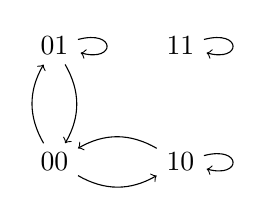
\begin{tikzpicture}[node distance=1cm and 1cm, every node/.style={scale=1.0}]
   \node[] (0) [] {00};
   \node[] (1) [above=of 0] {01};
   \node[] (2) [right=of 0] {10};
   \node[] (3) [above=of 2] {11};

   \draw[->] (0) edge [bend left] (1);
   \draw[->] (0) edge [bend right] (2);

   \draw[->] (1) edge [bend left] (0);
   \draw[->] (1) edge [loop right] (1);

   \draw[->] (2) edge [bend right] (0);
   \draw[->] (2) edge [loop right] (2);

   \draw[->] (3) edge [loop right] (3);
\end{tikzpicture}
\caption{State transition graph, under the fully asynchronous update.}%
\label{fig:stg}
\end{subfigure}\hfill%
\begin{subfigure}[b]{0.6\textwidth}
\centering
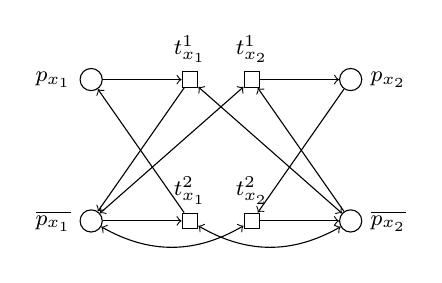
\begin{tikzpicture}[node distance=1cm and 1cm, every node/.style={scale=1.0}]\footnotesize
  \node[circle,draw,label=left:$p_{x_1}$] (x1) {};
  \node[circle,draw,label=left:$\overline{p_{x_1}}$] (nx1) [below=of x1, yshift=-0.5cm] {};

  \node[circle,draw,label=right:$p_{x_2}$] (x2) [right=of x1, xshift=2.0cm] {};
  \node[circle,draw,label=right:$\overline{p_{x_2}}$] (nx2) [below=of x2, yshift=-0.5cm] {};

  \node[rectangle,draw,label=above:$t^1_{x_1}$] (t1x1) [right=of x1] {};
  \node[rectangle,draw,label=above:$t^2_{x_1}$] (t2x1) [right=of nx1] {};

  \node[rectangle,draw,label=above:$t^1_{x_2}$] (t1x2) [left=of x2] {};
  \node[rectangle,draw,label=above:$t^2_{x_2}$] (t2x2) [left=of nx2] {};

  \draw[->] (x1) -- (t1x1);
  \draw[->] (t1x1) -- (nx1);
  \draw[<->] (t1x1) -- (nx2);

  \draw[->] (nx1) -- (t2x1);
  \draw[->] (t2x1) -- (x1);
  \draw[<->] (t2x1) edge [bend right] (nx2);

  \draw[->] (x2) -- (t2x2);
  \draw[->] (t2x2) -- (nx2);
  \draw[<->] (t2x2) edge [bend left] (nx1);

  \draw[->] (nx2) -- (t1x2);
  \draw[->] (t1x2) -- (x2);
  \draw[<->] (t1x2) -- (nx1);
\end{tikzpicture}
\caption{Petri net encoding of the model. Circles denote places, whereas rectangles denote transitions.}%
\label{fig:PN}
\end{subfigure}%
\caption{Dynamics and encoding of the Boolean network of Example~\ref{example:BN}}%
\label{fig:stg_and_PN}
\end{figure}

\subsection{Petri net encoding of Boolean networks}%
\label{sec:encoding}

\begin{definition}

  A \emph{Petri net} is a weighted bipartite directed graph \((P, T, W)\),
  where \(P\) is a non-empty finite set of vertices called \emph{places},
  \(T\) is a non-empty finite set of vertices called \emph{transitions},
  \(P \cap T = \emptyset\),
  and \(W : (P \times T) \cup (T \times P) \mapsto \mathbb{N} \) is a weight function attached to the arcs.

\end{definition}
A \emph{marking} for a Petri net is a mapping \(m : P \mapsto \mathbb{N}\) that assigns a number of tokens to each place. 
A place \(p\) is marked by a marking \(m\) if and only if \(m(p) > 0\). 
Marking \(m\) can be seen as a subset of \(P\) that contains all marked places by \(m\).
We shall write \(pred(x)\) (resp.\ \(succ(x)\)) to represent the set of vertices that have a (non-zero weighted) arc leading to (resp.\ coming from) \(x\).
In this work, we consider a class of Petri nets called 1-safe Petri nets where every place has at most 1 token and all arcs are of weight 1.
In this case, weights are implicitly omitted in the arcs of a Petri net.
Then, a transition \(t \in T\) is \emph{enabled} at a marking \(m\) if and only if \(pred(t) \subseteq m\). 
The firing of \(t\) leads to a new marking \(m'\) specified by \(m' = (m \backslash pred(t)) \cup succ(t)\).
Note that when multiple transitions are enabled, we need to embed one firing scheme (similar to the update scheme of a Boolean network) to the Petri net.
The classical firing scheme is that only one of the enabled transition is non-deterministically chosen to fire~\cite{Murata1989}.

The link between Boolean networks \emph{à la} Thomas and Petri nets was originally established in~\cite{chaouiya2004qualitative} in order to make available formal methods like model-checking for the analysis of such systems.
The basic encoding into 1-safe (i.e., never more than one token in each place) nets only holds for purely Boolean networks but was later extended to multivalued logical models in two ways, either in~\cite{chaouiya2011petri} with non 1-safe Petri nets or more recently in~\cite{chatain2014characterization} with 1-safe nets but many more places.

Since our study is focused on Boolean networks, we briefly recall the original encoding here.
Its basis is that every node (\emph{gene}) \(v\) of the original model \(\mathcal{N} = (V, F)\) is represented by two separate places (\(p_v\) and \(\overline{p}_v\)), corresponding to its two states, active, and inactive, respectively.
Each conjunct of the logical function that activates the \emph{gene} will lead to a transition \(t\), consuming the inactive place (i.e., a directional arc from \(\overline{p}_v\) to \(t\)), producing the active place (i.e., a directional arc from \(t\) to \(p_v\)), and with all other literals both consumed and produced (i.e., a bidirectional arc).
And conversely for the inactivation.
Let \(s\) be a state of the Boolean network and \(m_s\) be its corresponding marking in the encoded Petri net. 
It holds that \(\forall v \in V\), \(s(v) = 0\) if and only if \(m_s(\overline{p}_v) = 1\) and \(s(v) = 1\) if and only if \(m_s(p_v) = 1\). Note also that at any marking \(m\) of the Petri net encoding a Boolean network, it always holds that \(m(p_v) + m(\overline{p}_v) = 1\).

The main property of this encoding is that it is completely faithful with respect to the update scheme of the original Boolean network.
For each node \(v\) of \(\mathcal{N}\), only transitions corresponding to \(v\) can change the current marking of \(p_v\) or \(\overline{p_v}\).
In addition, at any marking at most one of such transitions is enabled because \(m(p_v) + m(\overline{p}_v) = 1\) holds.
Hence, for any update scheme in \(\mathcal{N}\), we have a corresponding firing scheme in \(\mathcal{P}\), which preserves the equivalence between the dynamics of \(\mathcal{N}\) and \(\mathcal{P}\)~\cite{DBLP:journals/nc/ChatainHKPT20}.

For illustration, let us reconsider the Boolean network shown in Example~\ref{example:BN}.
Figure~\ref{fig:PN} shows the Petri net encoding of this Boolean network.
Place \(p_{x_1}\) (resp. \(\overline{p_{x_1}}\)) in \(\mathcal{P}\) represents the activation (resp.\ the inactivation) of node \(x_1\) in \(\mathcal{N}\).
Marking \(\{p_{x_1}, \overline{p_{x_2}}\}\) in \(\mathcal{P}\) represents state 10 in \(\mathcal{N}\).
Transitions \(t^{1}_{x_1}\) and \(t^{2}_{x_1}\) represent the update of node \(x_1\).
Of course, in any marking \(t^{1}_{x_1}\) and \(t^{2}_{x_1}\) cannot be both enabled.
Then, the fully asynchronous update scheme in \(\mathcal{N}\) corresponds to the classical firing scheme in \(\mathcal{P}\) where only one of the enabled transitions for a given marking will be fired~\cite{Murata1989}.


Note that given a Boolean network in the standard SBML-Qual format~\cite{chaouiya2013sbml}, i.e., the package of SBML v3~\cite{keating2020sbml} for such models, one can easily obtain its Petri net encoding in the Petri Net Markup Language  (PNML)\footnote{\url{https://www.pnml.org/}} standard using the BioLQM\footnote{\url{http://www.colomoto.org/biolqm/}} library.
This piece of software extracted from GINsim~\cite{chaouiya2012logical} and part of the CoLoMoTo\footnote{\url{http://colomoto.org/}}~\cite{naldi2015cooperative} software suite allows for easy conversion between standard formats.
It also accepts many other common formats for Boolean networks, notably the \verb|.bnet| files of the  BoolNet~\cite{mussel2010boolnet,klarner2017pyboolnet} tools.
The conversion is executed as follows:

\noindent{\small \verb|java -jar GINsim.jar -lqm <input.{sbml,bnet,zginml,...}> <output.pnml>|}

Note that transforming a Boolean network defined by its functions into its Petri net encoding roughly relies on obtaining conditions for the activation and inactivation of the states. In~\cite{chaouiya2004qualitative} this took the form of the whole truth table of the Boolean functions, but as shown in Appendix 1 of~\cite{chatain2014characterization} computing Disjunctive Normal Forms (DNF) of each Boolean function is enough.
Though this might appear quite computationally intensive it is important to remark first that contrary to the prime-implicants case, there is no need to find \emph{minimal} DNFs.
One way to look at this is to consider that this amounts to a similar approach as that used in~\cite{DBLP:conf/ictai/ChevalierFPZ19} but with the encoding of both activation and inhibition functions as DNFs in order to take into account possible non-local-monotonicity.
This does not change the worst-case-complexity (obtaining a single DNF being exponential) but might matter a lot in practice.
As such, we will explore how this transformation, here using BDDs in BioLQM, and the one based on the most-permissive semantics compare in the Section~\ref{sec:eval} on evaluation.

\subsection{Siphons}

Siphons are a static and classical property of Petri nets~\cite{peterson1981petri}.
Note however that the use of siphons for the analysis of biological models, though it is not new, has been mostly relevant to the ODE-based continuous semantics of Chemical Reaction Networks~\cite{angeli2007petri,angeli2011persistence,degrand2020graphical}.

We recall here the basic definition establishing that to produce something in a siphon you must consume something from the siphon.
This corresponds to the idea that a siphon is a set of places that once unmarked remains unmarked.

\begin{definition}

  A \emph{siphon} of a Petri net \((P, T, W)\) is a set of places \(S\) such that:
  \[\forall t\in T, S\cap succ(t)\not =\emptyset\Rightarrow S\cap pred(t)\not =\emptyset.\]

\end{definition}

Note that \(\emptyset\) is trivially a siphon.

\section{Minimal trap spaces as maximal conflict-free siphons}
\label{sec:Main_finding}

First, we add a definition related to any set of places of a Petri net encoding a Boolean network, and notably a siphon of such a net.

\begin{definition}

  A set of places of Petri net \(\mathcal{P}\) encoding Boolean network \(\mathcal{M}\) is \emph{conflict-free} if it does not contain any two places corresponding to the active and inactive states of the same \emph{node} of \(\mathcal{N}\).
  Then, a conflict-free siphon \(S\) is said to be \emph{maximal} if and only if there is no other conflict-free siphon \(S'\) such that \(S \subset S'\).

\end{definition}

Intuitively, a siphon is a set of places that once unmarked remains so.
If it is conflict-free then its dual corresponds to a partial-state of the model such that whatever update, the fixed values remain so (since the unmarked places remain unmarked).
This is precisely the definition of a trap space and maximality of the siphon is equivalent to as many fixed values as possible, hence minimality of the trap space.
For example, the Boolean network given in Example~\ref{example:BN} has two trap spaces, \(m_1 = 11\) and \(m_2 = \star\star\).
The Petri net encoding of this Boolean network has five generic siphons, \(S_1 = \emptyset\), \(S_2 = \{p_{x_1}, \overline{p_{x_1}}\}\), \(S_3 = \{p_{x_2}, \overline{p_{x_2}}\}\), \(S_4 = \{\overline{p_{x_1}}, \overline{p_{x_2}}\}\), and \(S_5 = \{p_{x_1}, \overline{p_{x_1}}, p_{x_2}, \overline{p_{x_2}}\}\).
However, only \(S_1\) and \(S_4\) are conflict-free siphons and correspond to \(m_2\) and \(m_1\), respectively.
Since \(S_1 \subset S_4\), \(S_4\) is a maximal siphon corresponding to the minimal trap space \(m_1\).
Hereafter, we formally prove that a maximal conflict-free siphon is equivalent to a minimal trap space.

\begin{definition}

  Let \(m\) be a subspace of Boolean network \(\mathcal{N} = (V, F)\). 
  A \emph{mirror} of \(m\) is a set of places \(S\) in the Petri net encoding \(\mathcal{P}\) of \(\mathcal{N}\) such that:
  \[\forall v \in D_m, m(v) = 0 \Leftrightarrow p_v \in S, m(v) = 1 \Leftrightarrow \overline{p}_v \in S\] and \[\forall v \in V \setminus D_m, p_v \not \in S, \overline{p}_v \not \in S.\]

\end{definition}

\begin{theorem}%
\label{theo:ts_2_sp}

  Let \(\mathcal{M} = (V, F)\) be a Boolean network and \(\mathcal{P}\) be its Petri net encoding. A subspace \(m\) is a trap space of \(\mathcal{M}\) if and only if its mirror \(S\) is a conflict-free siphon of \(\mathcal{P}\).

\end{theorem}

\begin{proof}

  First, we show that if \(m\) is a trap space of \(\mathcal{M}\), then \(S\) is a conflict-free siphon of \(\mathcal{P}\) (*). If \(D_m = \emptyset\), then \(S = \emptyset\) is trivially a conflict-free siphon of \(\mathcal{P}\). Thus, we consider the case that \(D_m \neq \emptyset\) (resp. \(S \neq \emptyset\)). Assume that \(S\) is not a siphon of \(\mathcal{P}\). Then, there is a transition \(t \in T\) such that \(S\cap succ(t)\not =\emptyset\) but \(S\cap pred(t)=\emptyset\). In other words, there is a place \(p \in S\) such that \(p \in succ(t)\) but \(p \not \in pred(t)\). Let \(v\) be the corresponding node in \(\mathcal{M}\) of \(p\). By the characterization of the encoding~\cite{chaouiya2004qualitative}, there is a directional arc from \(t\) to \(p\) and a directional arc from the complementary place of \(p\) to \(t\). Without loss of generality, we assume that \(p = p_v\), then there is a directional arc from \(t\) to \(p_v\) and a directional arc from \(\overline{p}_v\) to \(t\). In addition, there is also no arc or a bidirectional arc between \(t\) and another place rather than \(p_v\) and \(\overline{p}_v\). Thus, there is no connecting arc between \(t\) and any place in \(S \setminus \{p_v\}\) because \(S\cap pred(t)\not =\emptyset\). In \(\mathcal{S}_{\mathcal{M}}[m]\), a node in \(V \setminus D_m\) can receive any Boolean value. Hence, there is a state \(s \in \mathcal{S}_{\mathcal{M}}[m]\) such that \(m_s(p') = 1, \forall p' \in pred(t) \setminus \{\overline{p_v}\}\) where \(m_s\) is the corresponding marking in \(\mathcal{P}\) of \(s\). We also have \(m_s(p_v) = 0\), leading to \(m_s(\overline{p_v}) = 1\) by the characterization of the encoding~\cite{chaouiya2004qualitative}. Now, \(t\) is enabled at marking \(m_s\). Its firing leads to a new marking \(m'_s\) such that \(m'_s(p_v) = 1\) and \(m'_s(\overline{p}_v) = 0\). Let \(s'\) be the corresponding state in \(\mathcal{M}\) of \(m'_s\). Since \(m\) is a trap space of \(\mathcal{M}\), \(s' \in \mathcal{S}_{\mathcal{M}}[m]\). Then, \(s'(v) = m(v)\), leading to \(m'_s(p_v) = 0\), which is a contradiction. Hence, \(S\) is a siphon of \(\mathcal{P}\). By the definition of a mirror, \(S\) is also a conflict-free one.

  Second, we show that if \(S\) is a conflict-free siphon of \(\mathcal{P}\), then \(m\) is a trap space of \(\mathcal{M}\) (**). By the definition of a mirror, \(m\) is a subspace of \(\mathcal{M}\). Let \(s\) be an arbitrary state in \(\mathcal{S}_{\mathcal{M}}[m]\) and \(m_s\) be its corresponding marking in \(\mathcal{P}\). By the characterization of the encoding~\cite{chaouiya2004qualitative}, \(m_s(p) = 0, \forall p \in S\). In any marking \(m'_s\) reachable from \(m_s\) regardless of the firing scheme of \(\mathcal{P}\), we have \(m'_s(p) = 0, \forall p \in S\) by the dynamical property on markings of a siphon~\cite{DBLP:journals/isci/LiuB16}. Equivalently, in any state \(s'\) reachable from \(s\) regardless of the update scheme of \(\mathcal{M}\), we have \(s'(v) = s(v) = m(v), \forall v \in D_m\). Then, \(s' \in \mathcal{S}_{\mathcal{M}}[m]\). By the definition of a trap space and the arbitrariness of \(s\), \(m\) is a trap space of \(\mathcal{M}\).

  From (*) and (**), we can conclude the proof.
\end{proof}

\begin{theorem}%
\label{theo:min_ts_2_max_sp}

  Let \(\mathcal{M}\) be a Boolean network and \(\mathcal{P}\) be its Petri net encoding. A subspace \(m\) is a minimal trap space of \(\mathcal{M}\) if and only if its mirror \(S\) is a maximal conflict-free siphon of \(\mathcal{P}\).

\end{theorem}

\begin{proof}

  First, we show that if \(m\) is a minimal trap space of \(\mathcal{M}\), then \(S\) is a maximal conflict-free siphon of \(\mathcal{P}\) (*). Since \(m\) is a trap space of \(\mathcal{M}\), \(S\) is a conflict-free siphon of \(\mathcal{P}\) by Theorem~\ref{theo:ts_2_sp}. Assume that \(S\) is not maximal. Then, there is another conflict-free siphon \(S'\) such that \(S \subset S'\). By Theorem~\ref{theo:ts_2_sp}, there is a trap space \(m'\) corresponding to \(S'\). Following the definition of a mirror, \(\mathcal{S}_{\mathcal{M}}[m'] \subset \mathcal{S}_{\mathcal{M}}[m]\), thus \(m' < m\). This is a contradiction because \(m\) is a minimal trap space. Hence, \(S\) is a maximal conflict-free siphon of \(\mathcal{P}\).

  Second, we show that if \(S\) is a maximal conflict-free siphon of \(\mathcal{P}\), then \(m\) is a minimal trap space of \(\mathcal{M}\) (**). Since \(S\) is a conflict-free siphon of \(\mathcal{P}\), \(m\) is a trap space of \(\mathcal{M}\) by Theorem~\ref{theo:ts_2_sp}. Assume that \(m\) is not minimal. Then, there is another trap space \(m'\) such that \(m' < m\). In other words, \(\mathcal{S}_{\mathcal{M}}[m'] \subset \mathcal{S}_{\mathcal{M}}[m]\). Let \(S'\) be the mirror of \(m'\). \(S'\) is a conflict-free siphon by Theorem~\ref{theo:ts_2_sp}. Following the definition of a mirror, \(S \subset S'\), which is a contradiction because \(S\) is a maximal conflict-free siphon. Hence, \(m\) is a minimal trap space of \(\mathcal{M}\).

  From (*) and (**), we can conclude the proof.
\end{proof}

We here showcase a theoretical application of the connection between trap spaces in Boolean networks and conflict-free siphons in Petri nets.
We use it to prove a property of minimal trap spaces, which has surprisingly not been formally proved.
Specifically, all minimal trap spaces of a Boolean network are mutually disjoint.
This property is important because we can use it to approximate the set of attractors of the Boolean network~\cite{klarner2015computing}.

\begin{theorem}%
\label{theo:separation_min_ts}

  Let \(\mathcal{N} = (V, F)\) be a Boolean network.
  For any two distinct minimal trap spaces \(m_1\) and \(m_2\) of \(\mathcal{N}\), we have that \(\mathcal{S}_{\mathcal{N}}[m_1] \cap \mathcal{S}_{\mathcal{N}}[m_2] = \emptyset\).

\end{theorem}

\begin{proof}

  Let \(\mathcal{P}\) be the Petri net encoding of \(\mathcal{N}\).
  If \(\mathcal{N}\) has only one minimal trap space, then the theorem trivially holds.
  Note that by Theorem~\ref{theo:min_ts_2_max_sp}, \(\mathcal{N}\) always has at least one minimal trap space because \(\mathcal{P}\) has at least one maximal conflict-free siphon.
  Hence, we consider the case that \(\mathcal{N}\) has at least two minimal trap spaces.

  Consider two any distinct minimal trap spaces \(m_1\) and \(m_2\).
  Assume that \(\mathcal{S}_{\mathcal{N}}[m_1] \cap \mathcal{S}_{\mathcal{N}}[m_2] \neq \emptyset\).
  Let \(S_1\) and \(S_2\) be the mirrors of \(m_1\) and \(m_2\), respectively.
  By Theorem~\ref{theo:min_ts_2_max_sp}, \(S_1\) and \(S_2\) are maximal conflict-free siphons of \(\mathcal{P}\).
  We have that \(S = S_1 \cup S_2\) is also a siphon because of the property of siphons in Petri nets~\cite{DBLP:journals/isci/LiuB16}.
  For every node \(v \in V\), assume that \(p_v \in S\) and \(\overline{p}_v \in S\) hold.
  Since \(S_1\) and \(S_2\) are conflict-free, there are all two cases.
  Case 1: \(p_v \in S_1\) and \(\overline{p}_v \in S_2\).
  Case 2: \(p_v \in S_2\) and \(\overline{p}_v \in S_1\).
  These two cases lead to \(m_1(v) \neq m_2(v), m_1(v) \neq \star, m_2(v) \neq \star\), then  \(\mathcal{S}_{\mathcal{N}}[m_1] \cap \mathcal{S}_{\mathcal{N}}[m_2] = \emptyset\).
  This is a contradiction.
  Hence, for every node \(v \in V\), \(p_v \in S\) and \(\overline{p}_v \in S\) cannot hold together.
  Therefore, \(S\) is conflict-free.
  Now, we have that \(S\) is a conflict-free siphon but \(S_1 \subset S\) or \(S_2 \subset S\) holds because \(S_1 \neq S_2\).
  This contradicts to the maximality of \(S_1\) and \(S_2\).
  Hence, \(\mathcal{S}_{\mathcal{N}}[m_1] \cap \mathcal{S}_{\mathcal{N}}[m_2] = \emptyset\) holds.
  
\end{proof}

As a computational application, by Theorem~\ref{theo:min_ts_2_max_sp}, we can reduce the problem of computing all minimal trap spaces of a Boolean network to the problem of computing all maximal conflict-free siphons of its Petri net encoding.
Note that in the case of special types of trap spaces (e.g., fixed points), this can be put in regard to special types of siphons in Petri nets.
See Subsection~\ref{subsec:computation_special_ts} for more discussions about many special types of trap spaces.
It might actually be possible to generalize our result to any 1-safe place-complementary Petri net to define a notion of trap spaces that might be useful for the analysis of Petri nets, but this is out of the scope of this article.

It is noted that there are no existing methods specifically designed for computing maximal conflict-free siphons (even maximal siphons) of a Petri net.
The reason might be that researchers mainly focus on minimal generic siphons~\cite{DBLP:journals/isci/LiuB16} in the field of Petri nets. 
Hence, we here propose several methods for computing maximal conflict-free siphons of a Petri net. 
The details of the proposed methods shall be given in the next section.

\section{Computation methods}
\label{sec:Computation}

\subsection{Characterization}
\label{subsec:siphon_characterization}

First, we show the characterization of all conflict-free siphons of the encoded Petri net \(\mathcal{P} = (P, T, W)\). Suppose that \(S\) is a generic siphon of \(\mathcal{P}\). If a place \(p\) should belong to \(S\), then by definition all the transitions in \(pred(p)\) must belong to \(succ(S)\). Note that \(succ(S) = \bigcup_{p \in S}succ(p)\). A transition \(t\) belongs to \(succ(S)\) if and only if there is at least one place \(p'\) in \(S\) such that \(p' \in pred(t)\). Hence, for each transition \(t \in pred(p)\), we can state that
\begin{equation}
\label{eq:siphon}
p \in S \Rightarrow \bigvee_{p' \in pred(t)}p' \in S.
\end{equation}
The system of all the rules of the above form with respect to all pairs \((p, t)\) where \(p \in P, t \in T, t \in pred(p)\) fully characterizes all generic siphons of a Petri net and has been used with SAT solvers in~\cite{oanea2010new,nabli2016enumerating}.
To make \(S\) to be a conflict-free siphon, we need to add to the system the rule
\begin{equation}
\label{eq:conflict}
p_v \in S \Rightarrow \overline{p_v} \not \in S \wedge \overline{p_v} \in S \Rightarrow p_v \not \in S
\end{equation}for each node \(v \in V\).
By definition, the final system fully characterizes all conflict-free siphons of the encoded Petri net.

\subsection{Constraint satisfaction problem}
\label{subsec:computation_csp}

The following Boolean Constraint Satisfaction Problem (CSP) directly derives from the above characterization:
\begin{definition}

  Given a Petri net \(\mathcal{P} = (P, T, W)\) encoding a Boolean network \(\mathcal{N} = (V, F)\).
  The CSP \(\mathcal{C}(\mathcal{P})\) is the triple \((R, D, C)\) where
  \begin{itemize}%
    \item \(R = P\), i.e., a variable is introduced for each place of \(\mathcal{P}\),
    \item \(D(p) = \mathbb{B}\) for all \(p \in R\), i.e., the variables are Boolean,
    \item \(C = \{\neg p_v \vee \neg \overline{p_v} = 1 \mid \forall v \in V\} \bigwedge
\{(p = 1 \rightarrow \bigvee_{p' \in pred(t)}p' = 1) \mid p \in P, t \in pred(p)\}\).
  \end{itemize}

\end{definition}

\begin{proposition}
\label{prop:csp_conflict_free_siphon}
  \(\mathcal{C}(\mathcal{P})\) is satisfied by a valuation \(r\) if and only if
  \[
    \{p \in P \;|\; r(p) = 1\}\
  \]
  is a conflict-free siphon of \(\mathcal{P}\).

\end{proposition}

\begin{proof}

  By the former part \(\neg p_v \vee \neg \overline{p_v}\) = 1 of \(C\), the conflict-freeness is imposed because for any satisfable valuation \(r\), \(r(p_v) = r(\overline{p_v}) = 1\) is impossible for all \(v \in V\).
  As shown in~\cite{nabli2016enumerating}, the latter part of \(C\) can characterize the set of all generic siphons of \(\mathcal{P}\).
  Hence, we can conclude the proof.
  
\end{proof}

In~\cite{nabli2016enumerating}, the set of all siphons of a given Petri net is characterized by a similar Boolean Constraint Satisfcation Problem (CSP) except the conflict-freeness constraint.
From the encoded CSP, the set of all \emph{minimal} siphons of the Petri net can be enumerated in the set inclusion order.
For enumerating siphons in the set inclusion order, the proposed method by~\cite{nabli2016enumerating} uses the technique that labels directly the Boolean variables with increasing value selection (i.e., to test first the absence, then the presence of a place in the candidate solution).
The method has two implementations, one uses an iterated SAT procedure and the other uses Constraint Logic Programming with backtracking.

One natural question is that how to use the CSP-based method for enumerating all the maximal conflict-free siphons of a Petri net encoding a Boolean model?
Of course, the set of all conflict-free siphons of the Petri net can easily characterized by the CSP model presented in~\cite{nabli2016enumerating} along with the additional constraint \(\neg p_v \vee \neg \overline{p_v} = 1\), for each \(v \in V\), which represents the conflict-freeness.
However, the main concern is to enumerate all the \emph{maximal} ones, which is not trivial to adapt from the CSP-based method.
By Proposition~\ref{prop:csp_conflict_free_siphon}, the set of all maximal conflict-free siphons of \(\mathcal{P}\) can be enumerated in the (maximality) set inclusion order, by restarting the search each time a conflict-free siphon \(S\) is found, with the following additional constraint for disallowing any subset of that conflict-free siphon: \(\bigvee_{p \not \in S} p = 1\).
For enumerating conflict-free siphons in the set inclusion order, we can use the same technique as used in~\cite{nabli2016enumerating} but with the opposite setting, i.e., labeling directly the Boolean variables with decreasing value selection.
The correctness of this technique comes from the fact that once \(S\) is found, it is the conflict-free siphon of maximum cardinality among all the remaining feasible conflict-free siphons.
Similar to~\cite{nabli2016enumerating}, the newly CSP-based method can also be implemented with SAT and CLP solvers.

However a more direct method is to use a MaxSAT solver.
We construct a MaxSAT problem with the following hard clauses:
\[
  (\neg p_v \vee \neg \overline{p_v}), \forall v \in V
\]
and
\[
  (\neg p \vee \bigvee_{p' \in pred(t)}p'), \forall p \in P, \forall t \in pred(p).
\]
We set a soft clause for each variable of the CSP and then use a ``minimal correction subset'' blocking strategy, which will ensure set-inclusion maximality of the solutions.
This is what is implemented in \texttt{trappist} using the RC2 MaxSAT solver~\cite{DBLP:journals/jsat/IgnatievMM19} available through the \texttt{python-sat} package\footnote{\url{https://pysathq.github.io/docs/html/api/examples/rc2.html}}.

\subsection{Answer set programming-based method}
\label{subsec:computation_asp}

Another possible method is to translate the characterization shown in Subsection~\ref{subsec:siphon_characterization} into the ASP \(\mathcal{L}\) as follows.
We introduce atom \verb|p-v| (resp. \verb|n-v|) to denote place \(p_v\) (resp. \(\overline{p_v}\)), \(\forall v \in V\). 
The set of all atoms in \(\mathcal{L}\) is given as \(\mathcal{A} = \bigcup_{v \in V}\{\verb|p-v|, \verb|n-v|\}\).
For each pair \((p, t)\) where \(p \in P, t \in T, t \in pred(p)\), we translate the rule (\ref{eq:siphon}) into the ASP rule
\[
\verb|a_1; ... ; a_k :- a.|
\]
where \(\verb|a| \in \mathcal{A}\) is the atom representing place \(p\) and \(\{\verb|a_1|, \dots,\verb|a_k|\} \subseteq \mathcal{A}\) is the set of atoms representing places in \(pred(t)\). The rule (\ref{eq:conflict}) is translated into the ASP rule
\[\verb|:- p-v, n-v.|\]
for each \(v \in V\). 
This ASP rule guarantees that two places representing the same node in \(\mathcal{M}\) never belong to the same siphon of \(\mathcal{P}\), representing the conflict-freeness.
Naturally, a Herbrand model (see, e.g.,~\cite{DBLP:journals/aicom/GebserKKOSS11}) of \(\mathcal{L}\) is equivalent to a conflict-free siphon of \(\mathcal{P}\).
To guarantee that a Herbrand model is also a stable model (an answer set), we need to add to \(\mathcal{L}\) the two choice rules
\[
\verb|{p-v}. {n-v}.|
\]
for each \(v \in V\).
Note that the number of atoms of \(\mathcal{L}\) is only \(2n\), whereas the ASP encoding shown in~\cite{klarner2015computing} has as many atoms as the number of prime-implicants of the Boolean network and that number might be exponential in \(n\).
In~\cite{DBLP:conf/ictai/ChevalierFPZ19}, there is an ASP characterization of trap spaces that does not rely on minimal DNFs either and thus seems very similar to our ASP encoding.
Remarkably it only requires the DNF for the \emph{activation} part, using the information that it will only be used for locally-monotonic Boolean networks.
We would therefore expect that, when available, it will have comparable performance on the ASP part (the ASP program would be approximately twice smaller, though redundancy is not always bad in that field), but can also avoid combinatorial explosion of the Petri net encoding for some formula where the activation DNF is simple but the inhibition is not.
Since mpbn is included in our benchmark this will be evaluated in our experiments.

Now, a solution (simply an answer set) \(A \subseteq \mathcal{A}\) of \(\mathcal{L}\) is equivalent to a conflict-free siphon \(S\) of \(\mathcal{P}\), thus a trap space \(m\) of \(\mathcal{M}\). The conversion from \(A\) to \(m\) is straightforward. If \(\verb|p-v| \in A\) then \(v \in D_m\) and \(m(v) = 0\). Conversely, if \(\verb|n-v| \in A\) then \(v \in D_m\) and \(m(v) = 1\). Otherwise, \(v \not \in D_m\). Computing multiple answer sets is built into ASP solvers and the solving collection POTASSCO~\cite{DBLP:journals/aicom/GebserKKOSS11} also features the option to find set-inclusion maximal answer sets with respect to the set of atoms. Naturally, a set-inclusion maximal answer set of \(\mathcal{L}\) is equivalent to a maximal conflict-free siphon of \(\mathcal{P}\), thus a minimal trap space of \(\mathcal{M}\). By using this built-in option, we can compute all the set-inclusion maximal answer sets of \(\mathcal{L}\) (resp.\ all the minimal trap spaces of \(\mathcal{M}\)) in one execution.

\subsection{Integer linear programming-based method}
\label{subsec:computation_ilp}

We first show how an Integer Linear Programming (ILP) \(\mathcal{I}\) can define a set of all conflict-free siphons of the encoded Petri net \(\mathcal{P}\).
We introduce \emph{binary} variable \verb|p-v| (resp. \verb|n-v|) to denote place \(p_v\) (resp. \(\overline{p_v}\)), \(\forall v \in V\).
The set of all binary variables in \(\mathcal{I}\) is \(\bigcup_{v \in V}\{\verb|p-v|, \verb|n-v|\}\).
For each pair \((p, t)\) where \(p \in P, t \in T, t \in pred(p)\), we translate the rule (\ref{eq:siphon}) into the ILP inequality
\[
\verb|a <= a_1 + ... + a_k|
\]
where \verb|a| is the binary variable representing place \(p\) and \{\verb|a_1|, \dots,\verb|a_k|\} is the set of binary variable representing places in \(pred(t)\).
The rule (\ref{eq:conflict}) is translated into the ILP inequality
\[\verb|p-v + n-v <= 1|\]
for each \(v \in V\).
This inequality forbids both \verb|p-v| and \verb|n-p| receive the value 1, thus representing the conflict-freeness.
Since we only consider feasible solutions, the objective function is set to \verb|max p-v| for some \(v \in V\).
Naturally, a solution \(I\) of \(\mathcal{I}\) is equivalent to a conflict-free siphon \(S\) of \(\mathcal{P}\).
The conversion is that
\[
  S = \{p \in P \;|\; I(\verb|a-p|) = 1\}
\]
where \verb|a-p| is the binary variable presenting place \(p\).

We can see the similarity between \(\mathcal{I}\) and the encoded ASP shown in the previous subsection.
However, due to the nature of solutions of an ILP, it is hard to compute all the set-inclusion maximal solutions of \(\mathcal{I}\) in one execution of an ILP solver.
Hence, we propose an iterative approach as follows.

The conflict-free siphon of maximum cardinality is of course maximal.
Therefore, we impose the following objective function:
\[
  \verb|max| \sum_{v \in V}(\verb|p-v| + \verb|n-v|).
\]
Now, \(\mathcal{I}\) can be solved using a general purpose ILP solver.
If it admits any solution \(I^{*}\), the corresponding conflict-free siphon (say \(S^{*}\)) is maximal.
Hence, it makes sense that it does not need to find any other conflict-free siphon of the net that is strictly contained in \(S^{*}\).
To do this, we add to \(\mathcal{I}\) a new inequality
\[
  \verb|1 <=| \sum_{p \in P \setminus S^{*}} \verb|a-p|
\]
where \verb|a-p| is the binary variable presenting place \(p\).
Now, we solve \(\mathcal{I}\) again to find a new solution.
If a new solution \(I'\) exists, then let \(S'\) be its corresponding conflict-free siphon.
Indeed, abide by the newly added inequality, we have \(S' \cap (P \setminus S^{*}) \neq \emptyset\) because there is some \verb|a-p| with \(p \in P \setminus S^{*}\) such that \(I'(\verb|a-p|) = 1\).
This implies that it is impossible that \(S' = S^{*}\) or \(S' \subset S^{*}\).
By the objective function, it means that \(S'\) is the conflict-free siphon of maximum cardinality among the conflict-free siphons that are not contained in \(S^{*}\).
Hence, \(S'\) is also a maximal conflict-free siphon.
Again, we add to \(\mathcal{I}\) a new inequality with respect to the newly found siphon.
The above process is iterated until \(\mathcal{I}\) becomes unfeasible, this means that there is no further maximal conflict-free siphon.
Thus, all the maximal conflict-free siphons of the Petri net have been found.

\subsection{Computation of special types of trap spaces}
\label{subsec:computation_special_ts}

\section{Motivating example}

% TODO Choose another motivating example because this Boolean model can be easily handled by mpbn 1.7

For a few years now we have been collaborating with biologists who build very large detailed and annotated maps and now wish to analyze the dynamics of the corresponding models.
One of the main maps studied this way represents knowledge about the Rheumatoïd Arthritis~\cite{singh2018computational}, and was the main motivation for the development of a tool to automatically transform it into an executable Boolean network~\cite{aghamiri2020automated}.
In the supplementary material of the paper, an excerpt of the map, focused around the apoptosis (cell death) module is transformed into a model of \emph{reasonable} size, namely 180 Boolean variables (model \verb|F5_RA_apoptosis_executable_module.sbml| of supplementary material S3, and model ``RA-apoptosis'' of Section~\ref{sec:eval}).
The study of such model, though, is a big hurdle.
Indeed, as stated in the article about another model of the same size:
\emph{``The size of the CaSQ-inferred MAPK model (181 nodes) made the calculation of stable states a non-realistic endeavour.''}

In practice, even if there is a huge number of attractors in such a model, obtaining a sample of those can reveal very useful to invalidate the model and lead to further refinement.
In particular, it provides a feature-rich alternative to random simulations for this type of very non-deterministic model.
Being able to detect that there are inconsistencies with published experimental data in some of the first 1000 attractors, for instance, can lead to a much quicker Systems Biology loop: model, invalidate, refine.

However, using a state-of-the-art tool like PyBoolNet~\cite{klarner2015computing} on that model actually fails at the phase of prime-implicant generation.
mpbn~\cite{Paulev2020} does not give any answer either because it recognizes that model as non-locally-monotonic.
And hence, it is not possible to extract any (complex) attractor at all.
This is also true for the Alzheimer model also mentioned in that same article and originally from~\cite{ogishima2016alzpathway} (\verb|F4| file in the original supplementary material, and ``Alzheimer'' in Table~\ref{tab:result_real}), but actually not for the MAPK model for which the first trap spaces can be obtained in reasonable time.
The current practice usually revolves then around fixing some inputs to plausible values and reducing the model accordingly.
While this approach makes sense, it relies on potentially arbitrary decisions, and \emph{hides away} critical modelling choices that were actually not part of the original Boolean network or even of the starting map.

Using the method presented above, it is possible to convert the model to PNML in about one second and to obtain the first 1000 minimal trap spaces (including ones that contain more than one state) in a few milliseconds.
Unfortunately since this was not available at the time, the analysis of the model remained very high-level and qualitative, instead of being able to use the rich information of computed minimal trap spaces.

\section{Evaluation}%
\label{sec:eval}

To assess the efficiency of the proposed method, implemented as a Python package named Trappist, we compared it with the state-of-the-art method implemented in the tool PyBoolNet~\cite{klarner2015computing,klarner2017pyboolnet} on both its own repository of models and large models from the literature.
In addition, we also included the tool mpbn~\cite{Paulev2020} to the benchmarks although it only handles locally-monotonic models, whereas both Trappist and PyBoolNet can handle general models.
To obtain a more comprehensive comparison, we also used random models generated by a third-party software (i.e., BoolNet R package~\cite{mussel2010boolnet}).

To solve the ASP problems, we used the same ASP solver CLINGO~\cite{DBLP:journals/aicom/GebserKKOSS11} and the same configuration as that used in PyBoolNet~\cite{klarner2015computing,klarner2017pyboolnet}.
Specifically, we used the configuration \texttt{-heuristic=Domain -enum-mod=domRec -dom-mod=3} (subset maximality, equivalent to the deprecated \texttt{--dom-pref=32 --heuristic=domain --dom-mod=7} used by PyBoolNet). We ran all the benchmarks on an apple laptop whose environment is CPU:\@ Intel\textregistered\ Core\texttrademark\ i7 1.20GHz x 4, 16 GB DDR4 RAM, MacOS 12.3.1. Finally, we set a time limit of two minutes for each model.
Note that we did not get the opportunity to run this benchmark on a proper dedicated computing workstation, the results are therefore only indicative of global trends and should not be interpreted as precise performance.
This is also why in some rare cases finding all minimal trap spaces was faster than with the limit to 1000.

For all the above tools, namely PyBoolNet, mpbn and CLINGO, we used the version available in the latest CoLoMoTo docker image tagged \texttt{2022-05-01}.
All the models and a CoLoMoTo notebook realizing the benchmarks can be found at \url{https://github.com/soli/trap-spaces-as-siphons}. These can be run on a Docker image in the cloud by clicking the ``Binder'' button.

\subsection{PyBoolNet repository}

\setlength{\tabcolsep}{4pt}
\begin{table}[!htb]
  \caption{Timing comparisons between bioLQM (LQM), PyBoolNet (PBN), mpbn and the four variants of Trappist on the PyBoolNet repository.}
  \centering%
  \label{tab:pyboolnet_repo}
  \begin{tabular}{rlrrrrrrrrr}
    \toprule
    & & & & & & & \multicolumn{4}{c}{Trappist}\\
    \cmidrule(rr){8-11}
    & model & \(n\) & \(|M|\) & LQM & PBN & mpbn & SAT & CLP & ILP & ASP \\
    \rownb & arellano\_rootstem & 9 & 4 & \textbf{0.13} & 0.05 & 0.01 & - & - & - & 0.02\\
    \rownb & calzone\_cellfate & 28 & 27 & \textbf{0.12} & 0.03 & \textbf{NM} & - & - & - & 0.03\\
    \rownb & dahlhaus\_neuroplastoma & 23 & 32 & \textbf{0.11} & 0.05 & 0.02 & - & - & - & 0.03\\
    \rownb & davidich\_yeast & 10 & 12 & \textbf{0.11} & 0.04 & 0.01 & - & - & - & 0.03\\
    \rownb & dinwoodie\_life & 15 & 7 & \textbf{0.11} & 0.03 & 0.01 & - & - & - & 0.03\\
    \rownb & dinwoodie\_stomatal & 13 & 1 & \textbf{0.10} & 0.03 & 0.01 & - & - & - & 0.02\\
    \rownb & faure\_cellcycle & 10 & 2 & \textbf{0.11} & 0.04 & 0.01 & - & - & - & 0.03\\
    \rownb & grieco\_mapk & 53 & 18 & \textbf{0.19} & 0.04 & 0.02 & - & - & - & 0.05\\
    \rownb & irons\_yeast & 18 & 1 & \textbf{0.12} & 0.05 & 0.01 & - & - & - & 0.03\\
    \rownb & jaoude\_thdiff & 103 & $>1000$ & N/A & \textbf{1.44} & \textbf{0.90} & - & - & - & 0.20\\
    \rownb & klamt\_tcr & 40 & 8 & 0.11 & 0.04 & 0.01 & - & - & - & 0.04\\
    \rownb & krumsiek\_myeloid & 11 & 6 & \textbf{0.10} & 0.03 & 0.01 & - & - & - & 0.02\\
    \rownb & multivalued & 13 & 4 & \textbf{0.10} & 0.03 & 0.01 & - & - & - & 0.02\\
    \rownb & n12c5 & 11 & 5 & 0.11 & \textbf{35.16} & 0.01 & - & - & - & 0.04\\
    \rownb & n3s1c1a & 2 & 2 & \textbf{0.10} & 0.02 & 0.01 & - & - & - & 0.02\\
    \rownb & n3s1c1b & 2 & 2 & \textbf{0.09} & 0.02 & 0.01 & - & - & - & 0.01\\
    \rownb & n5s3 & 4 & 3 & \textbf{0.10} & 0.03 & \textbf{NM} & - & - & - & 0.02\\
    \rownb & n6s1c2 & 5 & 3 & \textbf{0.10} & 0.03 & 0.01 & - & - & - & 0.02\\
    \rownb & n7s3 & 6 & 3 & \textbf{0.11} & 0.02 & 0.01 & - & - & - & 0.02\\
    \rownb & raf & 3 & 2 & \textbf{0.10} & 0.02 & 0.01 & - & - & - & 0.02\\
    \rownb & randomnet\_n15k3 & 15 & 3 & 0.10 & 0.03 & \textbf{NM} & - & - & - & 0.04\\
    \rownb & randomnet\_n7k3 & 7 & 10 & \textbf{0.10} & 0.03 & \textbf{NM} & - & - & - & 0.02\\
    \rownb & remy\_tumorigenesis & 34 & 25 & \textbf{0.15} & \textbf{2.14} & 0.02 & - & - & - & 0.06\\
    \rownb & saadatpour\_guardcell & 13 & 1 & \textbf{0.10} & 0.03 & 0.01 & - & - & - & 0.02\\
    \rownb & selvaggio\_emt & 56 & $>1000$ & N/A & \textbf{1.02} & \textbf{0.52} & - & - & - & 0.18\\
    \rownb & tournier\_apoptosis & 12 & 3 & \textbf{0.10} & 0.04 & 0.01 & - & - & - & 0.02\\
    \rownb & xiao\_wnt5a & 7 & 4 & \textbf{0.10} & 0.03 & 0.01 & - & - & - & 0.02\\
    \rownb & zhang\_tlgl & 60 & 156 & \textbf{0.60} & 0.22 & \textbf{NM} & - & - & - & 0.09\\
    \rownb & zhang\_tlgl\_v2 & 60 & 258 & \textbf{0.64} & 0.09 & 0.15 & - & - & - & 0.08\\
    \bottomrule
  \end{tabular}
\end{table}
\setcounter{rownumber}{0}

Column \(n\) denotes the number of nodes of each model. Column \(|M|\) denotes the number of minimal trap spaces and for each method is given the computation time in seconds, asking only for the first 1000 trap spaces.
A number in bold indicates a ratio greater than three compared to the best result. ``NM'' indicates a non-locally-monotonic model.
    
As shown in Table~\ref{tab:pyboolnet_repo}, for most of the models of the official PyBoolNet repository\footnote{\url{https://github.com/hklarner/pyboolnet/tree/master/pyboolnet/repository}}, the results are comparable with all minimal trap spaces found very fast.
For 5 of the 29 models, mpbn did not give any answer because it recognized these models as not locally-monotonic.
Note that on some very small models, Trappist is sometimes slower than PyBoolNet and/or mpbn, but still significantly under one second.
Moreover, we believe that the result on the arellano\_rootstem model is caused by the cold start of the JVM for BioLQM.\@
On the contrary, on every model that was a bit challenging for PyBoolNet or mpbn, the new method is far more efficient with speedups between one and two orders of magnitude.

\subsection{BBM repository}

\setlength{\tabcolsep}{4pt}
\begin{table}[!h]
  \caption{Results on the real-world models from the BBM repository.}
  \centering%
  \label{tab:bbm_repo}
  \begin{tabular}{l||r|r|r||r}
    \toprule
    Method & 1 min & 2 min & 3 min & Time average (s) \\ \midrule
    bioLQM & - & - & - & - \\
    PyBoolNet & - & - & - & - \\
    mpbn & - & - & - & - \\
    Trappist-maxSAT & - & - & - & - \\
    Trappist-CLP & - & - & - & - \\
    Trappist-ILP & - & - & - & - \\
    Trappist-ASP & - & - & - & - \\
    \bottomrule
  \end{tabular}
\end{table}
\setcounter{rownumber}{0}

\subsection{Selected models}

We used a set of real-world Boolean networks lying in various scales collected from numerous bibliographic sources.
These models are quite big (in size), complex (i.e., having high average in-degree, which is related to the number of prime-implicants) and most of them have never been fully analyzed.
We then applied PyBoolNet, mpbn, and Trappist to computing minimal trap spaces of these real-world models.
It is notable that unlike existing analysis shown in the literature, we did not fix specific values for source nodes (i.e., some node \(v\) such that \(f_v = v\)) in these models.
Table~\ref{tab:result_real} shows the experimental results on those models. Hereafter, we analyze in detail the results with respect to minimal trap space computation.

Column \(n\) (resp.\ \(s\)) denotes the number of nodes (resp.\ source nodes) of each model. Column \(|M|\) denotes the number of minimal trap spaces and for each method is given the computation time in seconds.
``DNF'' means that the method did not finish the computation (stopping at the first 1000 minimal trap spaces, or all for the last column) within the timeout of two minutes. ``NM'' indicates a non-locally-monotonic model.
    
\begin{table}[!htb]
  \caption{Timing comparisons between bioLQM (LQM), PyBoolNet (PBN), mpbn and the four variants of Trappist on selected models from the literature.}
  \centering%
  \label{tab:result_real}
  \begin{tabular}{rlrrrrrrrrr}
    \toprule
    & & & & & & & \multicolumn{4}{c}{Trappist}\\
    \cmidrule(rr){8-11}
    & model & \(n\) & \(|M|\) & LQM & PBN & mpbn & SAT & CLP & ILP & ASP \\
    \midrule % n < 100
    \rownb & Arabidopsis\_thaliana~\cite{DesignPrinciplesGeneNetworks} & 15 & 8 & 0.15 & - & - & - & - & - & - \\
    \rownb & Bcell~\cite{Dutta2019} & 73 & 72 & 0.21 & - & - & - & - & - & - \\
    \rownb & Cacace\_TdevModel~\cite{Cacace2020} & 61 & 28 & 1.21 & - & NM & - & - & - & - \\
    \rownb & Corral\_ThIL17diff~\cite{corral2021interplay} & 92 & - & N/A & - & - & - & - & - & - \\
    \rownb & DNA\_damage~\cite{DesignPrinciplesGeneNetworks} & 26 & - & 0.23 & - & NM & - & - & - & - \\
    \rownb & Drosophila~\cite{RodrguezVega2014} & 52 & - & 0.33 & - & - & - & - & - & - \\
    \rownb & EMT~\cite{Rozum2021} & 69 & - & - & - & - & - & - & - & - \\
    \rownb & mast\_cell~\cite{aghamiri2020automated} & 73 & - & N/A & - & - & - & - & - & - \\
    \rownb & FT-GRN~\cite{ChvezHernndez2022} & 23 & - & DNF & - & NM & - & - & - & - \\
    \rownb & hedgehog~\cite{DesignPrinciplesGeneNetworks} & 65 & - & N/A & - & - & - & - & - & - \\
    \rownb & metastatic~\cite{DesignPrinciplesGeneNetworks} & 10 & - & 0.11 & - & NM & - & - & - & - \\
    \rownb & Pancreatic\_Cancer~\cite{DesignPrinciplesGeneNetworks} & 43 & - & N/A & - & - & - & - & - & - \\
    \rownb & Pluripotent~\cite{DesignPrinciplesGeneNetworks} & 36 & - & 0.37 & - & NM & - & - & - & - \\
    \rownb & Rho-GTPases~\cite{DesignPrinciplesGeneNetworks} & 33 & 1 & 0.21 & - & - & - & - & - & - \\
    \rownb & Pluripotency~\cite{YachieKinoshita2018} & 36 & - & DNF & - & NM & - & - & - & - \\
    \rownb & p53\_high\_dna~\cite{DesignPrinciplesGeneNetworks} & 16 & 1 & 0.40 & - & NM & - & - & - & - \\
    \rownb & p53\_low\_dna~\cite{DesignPrinciplesGeneNetworks} & 16 & 1 & 0.38 & - & NM & - & - & - & - \\
    
    \midrule % 100 <= n < 200
    \rownb & angiofull~\cite{Weinstein2017} & 142 & - & N/A & - & - & - & - & - & - \\
    %\rownb & COVID\_19 & 111 & - & N/A & - & - & - & - & - & - \\
    \rownb & EMT\_Mech~\cite{Sullivan2022} & 136 & - & DNF & - & - & - & - & - & - \\
    \rownb & EMT\_Mech\_TGFbeta~\cite{Sullivan2022} & 150 & - & DNF & - & - & - & - & - & - \\
    \rownb & MAPK~\cite{aghamiri2020automated} & 181 & - & N/A & - & - & - & - & - & - \\
    \rownb & macrophage~\cite{DesignPrinciplesGeneNetworks} & 136 & - & N/A & - & - & - & - & - & - \\
    \rownb & RA\_apoptosis~\cite{aghamiri2020automated} & 180 & - & N/A & - & - & - & - & - & - \\
    \rownb & Adhesion\_CIP~\cite{guberman2020boolean} & 121 & - & 57.33 & - & - & - & - & - & - \\
    \rownb & angiogenesis~\cite{DesignPrinciplesGeneNetworks} & 141 & - & N/A & - & - & - & - & - & - \\
    
    \midrule % 200 <= n
    \rownb & T-cell-co-receptor~\cite{DesignPrinciplesGeneNetworks} & 206 & - & N/A & - & - & - & - & - & - \\
    \rownb & Snf1-pathway~\cite{Lubitz2015} & 202 & - & N/A & - & - & - & - & - & - \\
    \rownb & Mycobacterium~\cite{DesignPrinciplesGeneNetworks} & 317 & - & N/A & - & - & - & - & - & - \\
    \rownb & Leishmania~\cite{DesignPrinciplesGeneNetworks} & 342 & - & N/A & - & - & - & - & - & - \\
    \rownb & TcellCheckPoint~\cite{hernandez2020computational} & 218 & - & N/A & - & NM & - & - & - & - \\
    \rownb & Cholocystokinin~\cite{aghamiri2020automated} & 383 & - & N/A & - & - & - & - & - & - \\
    \rownb & Alzheimer~\cite{aghamiri2020automated} & 762 & - & N/A & - & NM & - & - & - & - \\
    
    \bottomrule
  \end{tabular}
\end{table}

The first observation is that for 26 of the 33 models (more than 78\%), mpbn did not give any answer because it recognized that these models as not locally-monotonic.
For 6 of the 33 models where mpbn returned the answers, mpbn and Trappist are comparable in computation time, though surprisingly mpbn appears a bit slower on average.
Note however that mpbn was the only tool to provide a solution for the SN-5 model, thus confirming that if the activation function is in the right form, not having to compute the inactivation function's disjunctive normal form can render a difficult problem tractable.
However, since mbpn can handle only locally-monotonic models and Trappist can handle general models, it is difficult to further compare between them.
Hence, we focus on only comparisons between PyBoolNet and Trappist in the following observations.

The second observation is that the proposed method vastly outperforms PyBoolNet in computational time, on each and every model, and sometimes with orders of magnitude of difference (e.g., for most models in the 100--1000 nodes size range).
Note that for all the cases where PyBoolNet did not manage to finish before the timeout, as marked by ``DNF'' in Table~\ref{tab:result_real}, the timeout occurred during the computation of the prime-implicants.
Hence, not even a single minimal trap space was output by that method.
The computational advantage is therefore immediately a practical advantage since on the one hand the state-of-the-art method did not allow any analysis whatsoever of the models, and on the other hand the proposed method could provide, very often under one second, the first thousand minimal trap spaces.
For modellers having a critical look at a model and in a \emph{model, invalidate, refine} loop this means a huge difference in the models that are amenable to study.

Note that even with a very restricted time-limit of two minutes, it was possible with the proposed technique to find \emph{all} minimal trap spaces of small models (roughly under 130 nodes, i.e., considered as quite big up to now).
Though it might seem impractical to handle tens of thousands of such possible complex attractors in a manual way, i.e., to compare them to specific experimental conditions and corresponding data, we hope that an automatic analysis of such attractors might become possible with systematic verification methods, not unlike that described in~\cite{hernandez2020computational}.
Since the ASP code is declarative by nature, it is also possible to add to it supplementary constraints coming from the modeler in case one is looking for specific attractors.
Finally, sampling from the ASP-generated solutions as is done in~\cite{chevalier2020synthesis} would allow for a different type of exploration.

The third observation is that for all the models where PyBoolNet finished before the timeout, once PyBoolNet went through the prime-implicant phase, its ASP solving phase quickly returned the first 1000 minimal trap spaces, all under one second.
For these models, the ASP solving phase of the proposed method also took very short time, all under one second.
Hence, with the experimental results shown in this paper, the practical differences between our ASP encoding and that of PyBoolNet are not distinctly exposed.
The fact that our new ASP encoding is guaranteed to be linear in the number of nodes of the original model does not seem to be crucial here, however a much deeper analysis of those cases remains to be done.

The last observation is that for very large models (i.e., more than two thousand nodes) the proposed method did not manage to finish the Petri net conversion before the timeout, as marked by ``???'' in Table~\ref{tab:result_real}.
This points to the fact that our current choice of using a BDD-based translation to obtain that Petri net encoding, though it provides a small/efficient ASP might be too costly to handle the largest models.
In such a case, a more \emph{naive} encoding might provide a much larger ASP program, with many redundant rules, but easier/faster to obtain.
The evaluation of the feasibility of such strategy, and of its impact on smaller instances, remains to be done and is out of the scope of this first article.
Recognizing that a model is locally-monotonic and applying in that specific case dedicated strategies as those of mpbn might also be a partial solution as shown in the SN-5 case, but not for the turei-2016 model.

Note that though enumerating the extremal siphons of a Petri net is exponential (see~\cite{nabli2016enumerating} for instance) this is apparently not the bottleneck of the proposed method, showing once again that networks obtained from biochemical models do have a specific structure.

\subsection{Randomly generated models}

\begin{table}[!htb]
  \caption{Results on N-K models.}
  \centering%
  \label{tab:result_N_K}
  \begin{tabular}{rrrrrrrr}
    \toprule
    & & & & \multicolumn{4}{c}{Trappist}\\
    \cmidrule(rr){5-8}
    \(n\) & LQM & mpbn & PBN & maxSAT & CLP & ILP & ASP \\
    \midrule
    100 & - & - & - & - & - & - & - \\
    150 & - & - & - & - & - & - & - \\
    200 & - & - & - & - & - & - & - \\
    250 & - & - & - & - & - & - & - \\
    300 & - & - & - & - & - & - & - \\
    350 & - & - & - & - & - & - & - \\
    400 & - & - & - & - & - & - & - \\
    \bottomrule
  \end{tabular}
\end{table}

\begin{table}[!htb]
  \caption{Results on scale-free models.}
  \centering%
  \label{tab:result_scale_free}
  \begin{tabular}{rrrrrrrr}
    \toprule
    & & & & \multicolumn{4}{c}{Trappist}\\
    \cmidrule(rr){5-8}
    \(n\) & LQM & mpbn & PBN & maxSAT & CLP & ILP & ASP \\
    \midrule
    500 & - & - & - & - & - & - & - \\
    750 & - & - & - & - & - & - & - \\
    1000 & - & - & - & - & - & - & - \\
    1250 & - & - & - & - & - & - & - \\
    1500 & - & - & - & - & - & - & - \\
    1750 & - & - & - & - & - & - & - \\
    2000 & - & - & - & - & - & - & - \\
    \bottomrule
  \end{tabular}
\end{table}

\section{Conclusion}

In this article we proposed a new method for the computation of minimal trap spaces of Boolean networks, based on a new concept called maximal conflict-free siphons.
This method is evaluated on large models from the literature and shows that it can scale up much better than the state-of-the-art prime-implicants based techniques.
We believe that this opens up the way to a much better analysis of large Boolean networks, which is needed with the advent of automatic model-generation pipelines~\cite{ostaszewski2021covid19}.

Though we benchmarked this new approach against state-of-the-art tools, there are many more evaluations that we plan to do in the future.
First, the BioLQM platform that we are using is providing another implicant-based method using BDDs in \url{http://colomoto.org/biolqm/doc/tools-trapspace.html} and though we expect it to behave mostly like PyBoolNet, that remains to be checked.
Note that this also raises the question of replacing altogether the BioLQM preprocessing step we use to obtain the Petri net encoding, since its use of BDDs might not be optimal for that step.
The trade-off between a small Petri net, and hence small ASP, and the time it takes to compute it (in other words, the trade-off of allowing redundant constraints) has to be evaluated in depth.

Second, the experimental results shown in this paper mostly expose the differences caused by the prime-implicant phase of PyBoolNet. There is much more information required to distinctly study the practical differences between our ASP encoding and that of PyBoolNet, and notably their size/efficiency ratio.
Hence, we plan to conduct experiments on more real-world models or maybe random models that can be randomly generated by using BoolNet~\cite{mussel2010boolnet}.
Such experiments should include a time-course of the number of ASP solutions found for proper comparison of the ASP encodings.

In addition, there are possibly other methods for computing maximal conflict-free siphons in Petri nets, like SAT/MaxSAT approaches~\cite{nabli2016enumerating}. Although these approaches do not directly support the maximal conflict-free siphon computation now, we plan to investigate them in the future. They could replace our ASP program if they outperform it.
However, the current method appears to already perform very well even on the biggest models we have considered.

Finally, we think that the links between Petri nets and Boolean networks that we stumbled upon in this method might have deeper roots. Exploring those connections might lead both to interesting topics of research for Petri nets, like a notion of trap-spaces, and for Boolean networks.

%% The Appendices part is started with the command \appendix;
%% appendix sections are then done as normal sections
%% \appendix

%% \section{}
%% \label{}

%% For citations use: 
%%       \citet{<label>} ==> Jones et al. [21]
%%       \citep{<label>} ==> [21]
%%

%% If you have bibdatabase file and want bibtex to generate the
%% bibitems, please use
%%
\bibliographystyle{elsarticle-num-names} 
\bibliography{tcs2022.bib}

%% else use the following coding to input the bibitems directly in the
%% TeX file.

% \begin{thebibliography}{00}

% %% \bibitem[Author(year)]{label}
% %% Text of bibliographic item

% \bibitem[ ()]{}

% \end{thebibliography}
\end{document}

\endinput
%%
%% End of file `elsarticle-template-num-names.tex'.
